
\section{Appendix}

\subsection{Adding New Geometric Types}\label{appdx:adding-new-geometric-types}

This section covers how to add new geometric types to the DDAD workbench.

\begin{enumerate}
  \item Create a new header and implementation file under the geometry library
  folder. See folder structure (\ref{appdx:folder-structure}). File names are in
  lower case with underscores between words (e.g. \texttt{geometry/my\_geometric\_type.h}.)
  Smaller, closely related items should be placed in the same file to avoid
  proliferation of tiny fragment files (e.g. polyline and polygon types are both placed into
  files named \texttt{polygon.h/polygon.cpp.}) See the coding
  guidelines (\ref{appdx:coding-guidelines}) for more detail on naming
  conventions.
  \item Define the interface of your new geometric type. You may use the
  template provided in listing~\ref{geometric-type-template} or look to existing
  geometric types for guidance.
  Importantly, you must inherit from \texttt{Visual::Geometry}. Some things you
  should notice about the template:
  \begin{itemize}
    \item All files start with the license (\ref{appdx:license}). 
    \item Next is a short one-liner describing the file that uses the
    \href{http://www.stack.nl/~dimitri/doxygen/}{Doxygen} tag \texttt{@brief}.
    \item All header files use
    \href{http://en.wikipedia.org/wiki/Include\_guard}{include guards}. Include
    guards in the geometry project are prefixed with \texttt{GE\_} and workbench
    include guards are prefixed with \texttt{WB\_}. Next, add the name of your
    file in uppercase. All guards end with \texttt{\_H}.
    \item All files include \texttt{common.h} which includes system utilities
    and logging. Visual types include \texttt{visual.h} which defines the visual
    geometry interfaces.
    \item Geometric types are suffixed with their dimension and the underlying
    arithmetic type. For example, \texttt{\_2f} denotes a 2 dimensional object
    with single-precision floating-point coordinates. See the coding
    guidelines (\ref{appdx:coding-guidelines}) for a full suffix listing.
  \end{itemize}
  \lstinputlisting[float, caption=Geometric Type Template,
  label=geometric-type-template]{code-samples/geometric-type-template.cpp}
  \item Provide implementations of the default constructor, copy constructor,
  and destructor. The copy constructor is important to implement if you plan on
  returning a copy of your type from functions, e.g. \texttt{Melkman} returns a
  \texttt{Polygon\_2r}. If you have not implemented a copy constructor, you may
  experience double-destruction of returned visualization primitives.
  \item Implement your geometric type as you normally would.
  \item Augment the type's methods with visual signals to reflect the state of
  the object. For example, listing~\ref{polyline-push-back} shows that adding a
  point to a polyline also registers the point so it can be viewed.
  \lstinputlisting[float, caption=Example of Augmented Method,
  label=polyline-push-back]{code-samples/polyline-push-back.cpp}
  \item Define a scene object (\ref{appdx:scene-objects}) type in
  \texttt{workbench/scene.h} that corresponds to your geometric type. You may
  use the template in listing~\ref{scene-object-template}.
  \lstinputlisting[float, caption=Scene Object Template,
  label=scene-object-template]{code-samples/scene-object-template.cpp}
  \item Implement the \texttt{Select}, \texttt{Deselect}, and \texttt{Intersect}
  methods so that your object can be selected in the editor. Refer to
  picking (\ref{appdx:picking}) for more details.
  \item Add a button to the Create tab defining ways for the user to create your
  object. Add the button using Qt Designer by opening
  \texttt{workbench/forms/window\_main.ui}. The button should have a
  human-readable name for your object and an icon representation. Add your
  button to the \texttt{buttonGroup} with \texttt{Right-click -> Assign to
  button group}.
  \item  Create a custom \texttt{MyGeometricObjectCreationMethod} widget. Click
  on \texttt{File -> New File or Project}. You will see the dialog shown in
  figure~\ref{fig:creation-method}.
  \begin{figure}[htb]
	\centering
	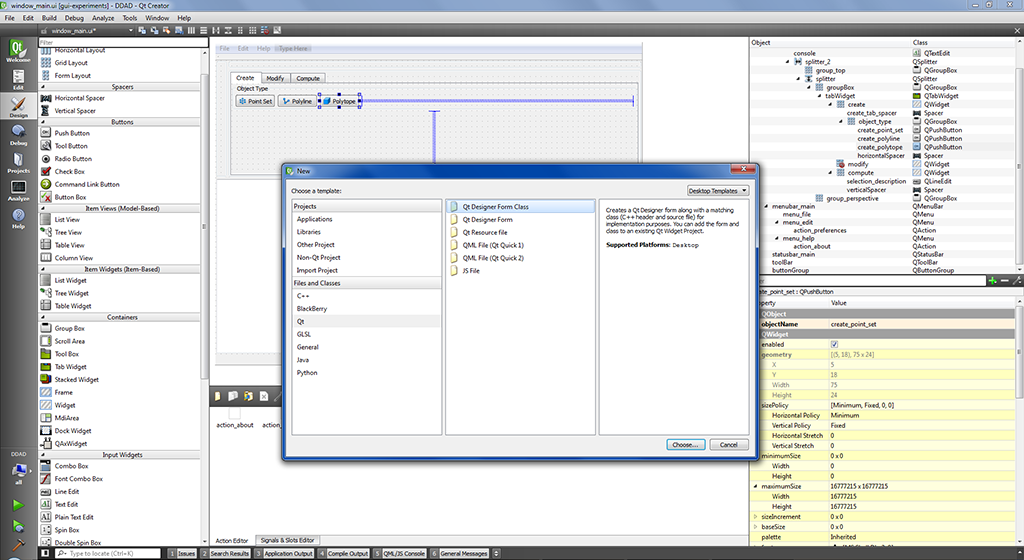
\includegraphics[width=\textwidth]{figures/gui-creation-method-new-file}
	\caption{Dialog for creating a new creation method widget.} 
	\label{fig:creation-method}
  \end{figure}
  \item Implement the \texttt{toggle} event handler for the button. Right-click
  on the button in Qt Designer and choose \texttt{Go to slot...} then
  \texttt{toggled(bool)}. This will automatically add the appropriate member
  functions onto the main window class and navigate you to the implementation
  stub in \texttt{qt\_window\_main.cpp}. Listing~\ref{creation-toggle-handler}
  shows the toggled handler for \texttt{Polyline\_2r} objects. Some things to notice:
  \lstinputlisting[float, caption=Creation Button Toggle Handler,
  label=creation-toggle-handler]{code-samples/creation-toggle-handler.cpp}
  \begin{itemize}
    \item All creation buttons must call \texttt{uncheckInputModeButtons()}
    since creation and input mode buttons are mutually exclusive.
    \item Use a static function variable for the \texttt{creation\_method}
    QWidget. The first time the button is \texttt{toggled(true)}, we create the
    widget and we destroy the widget when we are \texttt{toggled(false)}.
    \emph{Be sure to delete the widget to avoid a memory leak.}
    \item We set the input mode so that click events in the Orthographic Widget
    will be handled appropriately.
  \end{itemize}
\end{enumerate}




% 
% 1. Implement the `toggle` event handler for the button. Right-click on the button in Qt Designer and choose `Go to slot...` then `toggled(bool)`. This will automatically add the appropriate member functions onto the main window class and navigate you to the implementation stub in `qt_window_main.cpp`. Below is the toggled handler for Polyline_2r objects. Some things to notice:
% 
%   * All creation buttons must call `uncheckInputModeButtons()` since creation and input mode buttons are mutually exclusive. 
%   * Use a static function variable for the `creation_method` QWidget. The first time the button is `toggled(true)`, we create the widget and we destroy the widget when we are `toggled(false)`. _Be sure to delete the widget to avoid a memory leak._
%   * We set the input mode so that click events in the Orthographic Widget will be handled appropriately.
% 
%   ```C++
%   void MainWindow::on_create_polyline_toggled(bool checked) {
%       qDebug() << "on_create_polyline_toggled: " << checked;
% 
%       static PolylineCreationMethod *creation_method = nullptr;
% 
%       if (checked) {
%           ConfigManager::get().set_input_state(InputState::CREATE_POLYLINE);
%           uncheckInputModeButtons();
% 
%           creation_method = new PolylineCreationMethod();
% 
%           QLayoutItem *spacer = ui->create_tab_spacer;
%           ui->create->layout()->removeItem(spacer);
%           ui->create->layout()->addWidget(creation_method);
%           ui->create->layout()->addItem(spacer);
% 
%       } else if (creation_method) {
%           ui->create->layout()->removeWidget(creation_method);
%           delete creation_method;
%           creation_method = nullptr;
%       }
%   }
%   ```

\subsection{Coding Guidelines}\label{appdx:coding-guidelines}

Many organizations and individuals have taken the time to author style
guidelines for the C++ language. A thorough style document is an undertaking in
its own right; they may span many pages and include detailed rules, exceptions,
and justifications for both. For this project, it made sense to leverage the
work of others by adopting and customizing an existing set of guidelines.
\href{http://google-styleguide.googlecode.com/svn/trunk/cppguide.html}{Google's
C++ style guide}.

\emph{It is very important that contributors pay attention to coding style so
that we can keep the code uniform, clean, and easy to read.}

Some highlights:

\begin{itemize}
  \item Strictly adhere to 80-char line widths.
  \item Use lowercase, underscore separated variable names instead of
  camelCase.
  \item Private member variables should be suffixed with an underscore:
  \texttt{my\_member\_var\_}.
\end{itemize}

Some important additions or exceptions:

\begin{itemize}
  \item Geometric types are suffixed with their dimension and underlying
  arithmetic type.
  \begin{itemize}
    \item \texttt{f} = single-precision floating-point
    \item \texttt{d} = double-precision floating-point
    \item \texttt{i} = MPIR integer
    \item \texttt{r} = MPIR rational
  \end{itemize}
\end{itemize}
  

\subsection{Folder Structure}\label{appdx:folder-structure}

\subsection{Intersection Types}\label{appdx:intersection-types}

The geometry library defines a number of intersection types that represent the
intersection between two objects. It makes sense to create full types for
intersections because there is often quite a bit of information to capture (is
the intersection empty, a point, a line segment, a ray? when did the
intersection occur?). Perhaps more interestingly, intersection types nicely
align the C++ concept of constructors with our geometric concept of a
construction. The design is inspired by David Eberly's
\href{http://www.geometrictools.com/Source/Intersection2D.html}{geometric tools}.

Intersection types are placed in the \texttt{Intersection} namespace and follow
a naming convention: simply repeat the names of the two types being intersected.
The \texttt{Line\_2rLine\_2r} type is a good example:

\subsection{Picking}\label{appdx:picking}

\paragraph{The Problem.} Picking is the process of selecting the foremost object
in a view that lies under a user's mouse click. In our case, we are given an
input mouse click from either the orthographic or perspective views, and must
choose from among the scene objects.

\paragraph{Possible Solutions.}

\begin{enumerate}
  \item Color each object a unique color, render a frame, and use the
  final pixel color to determine which object to select. OpenGL provides a
  picking mode that does this.
  \item Generate a 3D world-space ray from the mouse click and intersect this
  ray with scene objects to determine which object it intersects first. 
\end{enumerate}

\paragraph{Our Solution.} We chose method 2 because it was more straightforward
to get working than 1 and probably more efficient. In particular, we take click
events from the orthographic and perspective views and convert them into a 3D
worldspace ray. We iterate over all scene objects (there is no hierarchical
acceleration structure) and produce \texttt{Ray\_3rSceneObject} intersection
objects. These objects are quite simple:

\subsection{License}\label{appdx:license}

\subsection{Scene Objects}\label{appdx:scene-objects}

% signals and slots
% configuration manager and input state
% 
% \subsection{Polyline2r}
% 
% Inside \texttt{qt\_window\_main.cpp}, we create a ``Create Polyline'' button and
% connect its triggered signal to the \texttt{onCreatePolylineTriggered} slot. We
% add this to the toolbar inside of a buttongroup with other buttons that are
% mutually exclusive (e.g. creating a polytope). The
% \texttt{onCreatePolylineTriggered} slot simply sets the input state to
% \texttt{CREATE\_POLYLINE}.
% 
% 
% 
% Handle ortho widget mouse clicks
% forward signals from ortho to scene observer
% 
% user must right-click in perspective to begin controlling camera. uses W S A D
% keys to move around.
% 
% 

% \subsection{Design and Implementation of Polyline and Polygon Types}
% \label{sec:polyline-polygon}
% 
% [todo - rework to be about design of a general polyline and polygon not
% specific to melkman]
% 
% The real work of implementing Melkman's algorithm is designing the data types
% upon which it operates. In particular, we require data types for two geometric
% objects: input polylines and output polygons. Beyond the standard concerns of
% efficiency and ease of use, both data types must support visualization and our
% polygon type must support deque semantics.
% 
% Our workbench provides an abstract data type, \texttt{Visual::Geometry}, that
% geometric data types can inherit to become \emph{visual geometry} types and gain
% access to the visualization system. We provide an in-depth discussion of how
% \texttt{Visual::Geometry} works in Section~\ref{sec:workbench-architecture}, but
% for now it is sufficient to know that uses the observer
% pattern~\cite{gamma1994design} to generate and recieve visual events. In
% particular, visual geometry objects are able to both observe visual geometry
% objects and to be observed by visual geometry objects. A visual geometry object
% may \emph{signal} to its observers that a visual event has occurred, and can
% optionally implement a \emph{slot} that handles signals from the objects that it
% observes. By default, visual geometry objects simply forward signals they
% recieve up to their observers, forming an event propagation chain.
% 
% 
% A major benefit of visual geometry types is their ability to offload
% visualization work through composition. Our polygon type must support deque
% operations, but we only require sequential access to the polyline's vertices. In
% our case, we can think of the polygon as being composed of a polyline boundary.
% This suggests using a deque as a backing store for the polyline's vertices so
% that the polygon type may simply delegate deque operations to its boundary. This
% choice is consistent with our need for constant sequential access to the
% polyline's vertices.
% 
% The \texttt{Polygon\_2r} class is composed of a \texttt{Polyline\_2r} boundary
% that is responsible for visualizing vertices and edges. It can optionally
% visualize the polygon interior by triangulating it into a fan. The
% \texttt{Polyline\_2r} class uses a deque to store its vertices. The
% \texttt{push\_back} and \texttt{pop\_back} methods are responsible for
% visualizing how those operations affect the visual state of the object.

%  We know from the algorithm description that these should support deque
% semantics, so it makes sense to use this as a backing store for the polygon's
% vertices. In many regards, a polygon will act like a polyline, e.g. we can add
% and remove vertices to both. In order to avoid duplicating functionality, it
% makes sense to compose our polygon with a polyline boundary and forward common
% events to it. We want to visualize both objects, so each will inherit from the
% Visual::Geometry class.
